% talk.tex -- student project kick-off, 28 October 2026
% Built from TOX-MD-presentation-guide.md (Section 4), one frame per slide.
% Build: latexmk -pdf talk.tex   (or pdflatex twice)
% Speaker notes: switch notes=none to notes=second (second screen) or notes=only.
% Fonts: the design font is Source Sans (font=source, needs the sourcesanspro package);
% font=helvet is used here because it is available everywhere.
\documentclass[aspectratio=169]{beamer}
\usepackage[lang=en, font=helvet, notes=none, nosectionslides]{thbtalk}
\usetikzlibrary{arrows.meta, positioning, calc}
\pgfplotsset{compat=1.16}

% Colour-blind-safe (Okabe-Ito); the same object keeps its colour throughout.
\definecolor{casecol}{HTML}{E69F00}    % case
\definecolor{ctrlcol}{HTML}{0072B2}    % control
\definecolor{nullcol}{HTML}{999999}    % null
\definecolor{obscol}{HTML}{CC79A7}     % observed
\definecolor{accentcol}{HTML}{009E73}  % neutral highlight
\newcommand{\case}{\textcolor{casecol}{\textbf{case}}}
\newcommand{\ctrl}{\textcolor{ctrlcol}{\textbf{control}}}

% Outlook timeline phases
\tikzset{ph/.style={fill=#1, rounded corners=2pt, minimum height=0.8cm, align=center, text=thbink}}

% Visible marker for everything the presenter still has to confirm or supply.
\newcommand{\todo}[1]{{\color{red}\bfseries[TODO: #1]}}

\title{Evaluating a multi-dimensional noise model for differential expression in multi-tissue RNA-seq data}
\subtitle{Student project kick-off}
\author[Aaron Schröder]{Project Lead: Aaron Schröder}
\institute{TH Bingen -- aaron.schroeder@th-bingen.de}
\date{28 October 2026}

\begin{document}

% ============================================================== opening
% ---------------------------------------------------------------- 1
\thbtitleframe

% ---------------------------------------------------------------- 2
\section{Scientific question}
\begin{frame}{Agenda}
  \begin{enumerate}
    \item Scientific question
    \item Material: biology and the data we use
    \item Methods: the noise model and how to evaluate it
    \item Data: what is available, what is expected
    \item First steps: the first two weeks
    \item Outlook: the coming months
  \end{enumerate}
  \note{Six items, exactly the organizers' list. About 40 minutes, questions welcome at any time.}
\end{frame}

% ---------------------------------------------------------------- 3
\begin{frame}{Scientific question}
  \begin{keyeq}
    Does the multi-dimensional TOX model control false positives,\\
    and how does its power compare with limma, edgeR and DESeq2?
  \end{keyeq}
  \vspace{1em}
  \begin{twocols}
    \textbf{Calibration:} are the p-values honest?
    \colbreak
    \textbf{Power:} does it find true effects?
  \end{twocols}
  \note{Two parts. Calibration: if nothing changes, does the test say so at the advertised rate?
    Power: when something does change, how often is it found?
    Result for you: a reproducible evaluation that shows where the model is reliable and where it is not.
    A negative result is a valid result.}
\end{frame}

% ============================================================== primers
% ---------------------------------------------------------------- 4
\section{Material}
\begin{frame}{Biology primer: gene expression and RNA-seq}
  \begin{itemize}
    \item gene $\rightarrow$ RNA $\rightarrow$ protein; expression = how much RNA
    \item RNA-seq: one read \textbf{count} per gene per sample
    \item replicates: independent samples of the same condition
    \item sequencing depth differs between samples $\Rightarrow$ normalization
  \end{itemize}
  \vspace{0.6em}
  {\centering\resizebox{0.95\linewidth}{!}{% F1: RNA-seq pipeline, tissue sample -> sequencing -> count matrix (schematic)
\begin{tikzpicture}[
    stage/.style={draw=thbline, fill=thbtint, rounded corners=2pt, align=center,
                  minimum height=1.25cm, text width=2.15cm, font=\footnotesize},
    arr/.style={-{Stealth[length=2.2mm]}, thick, thbmuted}]
  \node[stage] (s) {tissue sample\\[1pt]{\scriptsize case or control}};
  \node[stage, right=0.55cm of s] (r) {extract RNA};
  \node[stage, right=0.55cm of r] (q) {sequence\\[1pt]{\scriptsize millions of reads}};
  \node[stage, right=0.55cm of q] (m) {map \& count\\[1pt]{\scriptsize reads per gene}};
  \draw[arr] (s) -- (r);
  \draw[arr] (r) -- (q);
  \draw[arr] (q) -- (m);
  % count matrix: genes x samples
  \begin{scope}[shift={($(m.east)+(0.75cm,-0.95cm)$)}, font=\scriptsize]
    \foreach \j/\c in {1/casecol,2/casecol,3/casecol,4/ctrlcol,5/ctrlcol,6/ctrlcol} {
      \fill[\c!35] (0.42*\j-0.42,1.9) rectangle ++(0.42,0.22);
    }
    \foreach \i/\row in {0/{812,640,955,121,97,140},1/{3,0,5,2,1,4},2/{57,61,49,58,66,52},3/{0,1,0,410,388,452}} {
      \foreach \v [count=\j] in \row {
        \node[anchor=center, text=thbink] at (0.42*\j-0.21,1.62-0.42*\i) {\v};
      }
    }
    \draw[thbline] (0,0) rectangle (2.52,1.9);
    \node[anchor=south, text=thbmuted] at (1.26,2.12) {samples};
    \node[anchor=south, rotate=90, text=thbmuted] at (-0.05,0.95) {genes};
    \node[anchor=north, text=thbmuted, align=center] at (1.26,-0.05) {count matrix\\(illustrative numbers)};
  \end{scope}
  \draw[arr] (m.east) -- ++(0.3cm,0);
\end{tikzpicture}
}\par}
  \note{A gene is transcribed into RNA; RNA-seq counts the RNA fragments of each gene.
    The result is a count matrix: genes in rows, samples in columns.
    Counts are not directly comparable between samples: a sample sequenced twice as deep has
    roughly twice the counts. Hence normalization: TMM (edgeR) and median-of-ratios (DESeq2) for
    counts; TPM as a within-sample scale.
    Replicates are independent biological samples of the same condition; they tell us how much
    expression varies naturally.
    Expression is tissue specific: photosynthesis genes are high in leaf and near zero in root.
    No library preparation details needed for this project.}
\end{frame}

% ---------------------------------------------------------------- 5
\begin{frame}{Case vs control, across tissues}
  \begin{twocols}[0.46]
    \begin{itemize}
      \item contrast: \case\ vs \ctrl
      \item effect: log2 fold change (log2FC)
      \item one gene, $d$ tissues $\Rightarrow$ a \textbf{vector} of effects
      \item question: does the gene respond \emph{anywhere}?
    \end{itemize}
    \colbreak
    % F2: one gene's log2FC across three tissues (illustrative values, not data)
\begin{tikzpicture}
  \begin{axis}[thbplot, width=0.95\linewidth, height=0.5\textheight,
      ybar, bar width=0.9cm, grid=none, ymin=-1, ymax=2.6,
      symbolic x coords={leaf,stem,root}, xtick=data,
      ylabel={log2 fold change (case / control)},
      extra y ticks={0}, extra y tick style={grid=major, grid style={thbmuted}},
      title={\footnotesize\color{thbmuted}one gene, three tissues (illustrative)}]
    \addplot[fill=casecol, draw=none] coordinates {(leaf,2.1) (stem,0.15) (root,-0.2)};
  \end{axis}
\end{tikzpicture}

  \end{twocols}
  \note{log2FC of 1 means doubled, -1 halved, 0 unchanged.
    The gene on the right responds in leaf and hardly at all in stem and root.
    A per-tissue test asks three separate questions. The multi-dimensional test asks one: is the
    gene's whole response vector larger than noise? That is why we need a multi-dimensional test.
    The bar values are illustrative, not data.}
\end{frame}

% ---------------------------------------------------------------- 6
\section{Methods}
\begin{frame}{Statistics primer}
  \begin{columns}[T,onlytextwidth]\begin{column}{0.3\textwidth}
    \begin{itemize}
      \item null distribution
      \item p-value
      \item calibration
      \item FDR (Benjamini--Hochberg)
      \item power (TPR)
    \end{itemize}
  \end{column}\hfill\begin{column}{0.66\textwidth}
    \resizebox{\linewidth}{!}{% F6: what calibration looks like. ILLUSTRATIVE shapes, not data.
% (a) null p-value histogram, 10 bins: flat (calibrated) vs spike at 0 (anti-conservative).
% (b) observed vs nominal FDR: diagonal (honest) vs 1.6 x nominal (too liberal).
\begin{tikzpicture}[font=\footnotesize]
  % ---------------- (a) histogram: x 0..1 -> 0..5 cm, density 0..2.4 -> 0..3.6 cm
  \begin{scope}
    \foreach \i in {0,...,9} \fill[nullcol!45] (0.5*\i+0.03,0) rectangle (0.5*\i+0.47,1.5);
    \draw[obscol, very thick]
      (0,0) -- (0,3.3) -- (0.5,3.3) -- (0.5,1.95) -- (1,1.95) -- (1,1.5) -- (1.5,1.5)
      -- (1.5,1.35) -- (2,1.35) -- (2,1.275) -- (2.5,1.275) -- (2.5,1.2) -- (3.5,1.2)
      -- (3.5,1.125) -- (4,1.125) -- (4,1.05) -- (5,1.05) -- (5,0);
    \draw[thbmuted] (0,0) -- (5.1,0);
    \draw[thbmuted] (0,0) -- (0,3.7);
    \foreach \x/\l in {0/0,2.5/0.5,5/1} \node[anchor=north, text=thbmuted] at (\x,0) {\l};
    \foreach \y/\l in {0/0,1.5/1,3/2} \node[anchor=east, text=thbmuted] at (0,\y) {\l};
    \node[anchor=north, text=thbmuted] at (2.5,-0.4) {p-value};
    \node[anchor=south, rotate=90, text=thbmuted] at (-0.45,1.8) {density};
    \node[anchor=south] at (2.5,3.8) {(a) p-values under the null};
    \fill[nullcol!45] (2.3,3.0) rectangle ++(0.3,0.2);
    \node[anchor=west] at (2.65,3.1) {calibrated};
    \draw[obscol, very thick] (2.3,2.55) -- ++(0.3,0);
    \node[anchor=west] at (2.65,2.55) {anti-conservative};
  \end{scope}
  % ---------------- (b) FDR: nominal 0..0.2 -> 0..4 cm, observed 0..0.3 -> 0..3.6 cm
  \begin{scope}[xshift=7cm]
    \draw[thbline] (0,0) grid[xstep=1, ystep=1.2] (4,3.6);
    \draw[nullcol, very thick, dashed] (0,0) -- (4,2.4);
    \draw[obscol, very thick] (0,0) -- (3.75,3.6) -- (4,3.6);
    \draw[thbmuted] (0,0) -- (4.1,0);
    \draw[thbmuted] (0,0) -- (0,3.7);
    \foreach \x/\l in {0/0,1/0.05,2/0.1,4/0.2} \node[anchor=north, text=thbmuted] at (\x,0) {\l};
    \foreach \y/\l in {0/0,1.2/0.1,2.4/0.2,3.6/0.3} \node[anchor=east, text=thbmuted] at (0,\y) {\l};
    \node[anchor=north, text=thbmuted] at (2,-0.4) {nominal FDR};
    \node[anchor=south, rotate=90, text=thbmuted] at (-0.75,1.8) {observed FDR};
    \node[anchor=south] at (2,3.8) {(b) observed vs nominal FDR};
    \node[anchor=west, text=nullcol!80!black] at (2.6,1.4) {honest};
    \node[anchor=east, text=obscol] at (2.1,2.6) {too liberal};
  \end{scope}
  \node[anchor=north, text=thbmuted, font=\scriptsize] at (5.5,-1.05) {illustrative shapes, not data};
\end{tikzpicture}
}
  \end{column}\end{columns}
  \note{Null distribution: what the statistic looks like when nothing changes.
    p-value: how extreme the observation is under the null.
    Under the null, p-values are uniform (left, grey). A spike at 0 (purple) means too many small
    p-values: anti-conservative.
    Calibration: the false-positive rate at a threshold matches the threshold.
    Benjamini--Hochberg controls the FDR, the expected share of false discoveries among the calls.
    Right: an honest method lies on the diagonal.
    Power is the share of true effects found (TPR).
    Important: a method can look powerful because it is anti-conservative, so power is only
    meaningful together with calibration. Both plots are illustrative shapes, not data.}
\end{frame}

% ---------------------------------------------------------------- 7
\begin{frame}{Existing tools}
  \begin{tabular}{lll}
    \toprule
    \thbhead{Tool} & \thbhead{Noise model} & \thbhead{Variance estimate} \\
    \midrule
    edgeR  & negative binomial on counts & dispersion, empirical Bayes shrinkage \\
    DESeq2 & negative binomial on counts & dispersion, shrunk towards a mean trend \\
    limma  & linear model on log values  & empirical Bayes moderation \\
    \bottomrule
  \end{tabular}
  \vspace{0.8em}
  \begin{itemize}
    \item multi-tissue: \textbf{no obvious 1:1 reference} -- part of your task
  \end{itemize}
  \note{Each tool assumes a noise model. They are well validated; we do not claim they fail.
    The open question is the multi-tissue setting and what a non-parametric empirical null does there.
    Candidate ideas for a multi-tissue comparison, not recommendations:
    (1) omnibus tests in a tissue-by-condition design: moderated F-test in limma, quasi-likelihood
    F-test in edgeR, likelihood-ratio test in DESeq2. They ask "any effect in any tissue"; TOX uses
    the norm of the effect vector.
    (2) combining per-tissue p-values (e.g. Simes, Sidak).
    (3) limma::fry() and edgeR::diffSpliceDGE(); limma's counterpart of the latter is diffSplice().
    fry is a gene-set test and returns set-level p-values, no per-gene effects; diffSpliceDGE tests
    whether effects differ between the exons of a gene, i.e. a relative effect. Both answer related
    but different questions. Your task: assess whether these approaches and comparisons are feasible
    per gene across tissues, and what their limitations are.
    There will be no 1:1 comparability; look for the limitations of each approach.}
\end{frame}

% ---------------------------------------------------------------- 8
\begin{frame}{The TOX idea (one tissue)}
  \begin{columns}[T,onlytextwidth]\begin{column}{0.37\textwidth}
    \begin{itemize}
      \item estimate the noise \textbf{from the data}
      \item neighbours: genes with a similar mean
      \item pool their residuals
      \item read the null off the pool
    \end{itemize}
  \end{column}\hfill\begin{column}{0.6\textwidth}
    \resizebox{\linewidth}{!}{% F3: residuals against gene mean, with the neighbourhood of one target gene (schematic).
% Pseudo-random but fixed points (seeded), spread growing with the mean. Not data.
\begin{tikzpicture}[x=0.36cm, y=1.1cm]
  \pgfmathsetseed{185}
  % neighbourhood window around the target gene (gene 14)
  \fill[thbtint] (11.5,-1.75) rectangle (16.5,1.75);
  \draw[thbprimary, dashed] (11.5,-1.75) -- (11.5,1.75) (16.5,-1.75) -- (16.5,1.75);
  \draw[thbmuted] (0,0) -- (28.5,0);
  \draw[-{Stealth}, thbmuted] (0,-1.8) -- (0,1.95);
  \draw[-{Stealth}, thbmuted] (0,-1.8) -- (28.8,-1.8);
  \node[anchor=north, font=\scriptsize, text=thbmuted] at (14.4,-1.85) {gene mean (genes sorted by mean)};
  \node[anchor=south, rotate=90, font=\scriptsize, text=thbmuted] at (-0.2,0) {residual};
  \foreach \g in {1,...,27} {
    \pgfmathsetmacro{\s}{0.25+0.045*\g}
    \foreach \r in {1,2,3} {
      \pgfmathsetmacro{\e}{\s*rand}
      \ifnum\g>11 \ifnum\g<17
        \fill[casecol] (\g,\e) circle (2.6pt);
      \else
        \fill[casecol!35] (\g,\e) circle (2pt);
      \fi\else
        \fill[casecol!35] (\g,\e) circle (2pt);
      \fi
    }
  }
  \draw[thbprimary, thick] (14,-1.6) -- (14,1.6);
  \node[anchor=south, font=\scriptsize, text=thbprimary] at (14,1.75) {target gene};
  \node[anchor=north west, font=\scriptsize, text=thbprimary, align=left] at (16.7,1.7)
       {neighbours: genes with\\similar mean (k genes)};
\end{tikzpicture}
}
    {\centering\scriptsize\color{thbmuted} schematic: one group (e.g.\ case); not data\par}
  \end{column}\end{columns}
  \note{For a gene, find neighbour genes with a similar mean expression and collect their
    within-group residuals: replicate minus group mean. These residuals form the empirical noise
    distribution. Neighbours are found separately for case and control, each on its own group mean.
    No parametric count distribution is assumed. The assumption is that genes with similar group
    means have exchangeable within-group residuals.
    Do not call it distribution-free or assumption-free.
    Source: misc/Tensor_Omics_Methods/Empirical_Noise-Based_Significance_of_Distances.tex.}
\end{frame}

% ---------------------------------------------------------------- 9
\begin{frame}{1-D mechanics}
  \begin{enumerate}
    \item group means per gene (case, control)
    \item residual pool: adaptive kNN, counted in \textbf{genes}
    \item scale each pool by $1/\sqrt{n}$ of its own group
    \item null of the mean difference: all case--control residual pairs
    \item p-value from the tail count
  \end{enumerate}
  \note{Step 3: the observed statistic is a difference of means over n replicates; one residual is at
    single-observation scale. Scaling by 1/sqrt(n) of its own group puts it on the scale of a mean.
    Step 2: the neighbourhood starts at the gene with the closest mean and grows outward in sorted-mean
    order to k\_start genes; then k\_step genes at a time while the mean absolute residual of the pool
    grows by no more than tau (relative), up to k\_max genes. Residuals carry a Bessel correction
    sqrt(n/(n-1)).
    Step 4 and 5 describe the exact module: every case-pool residual paired with every control-pool
    residual, counted exactly by sorted binary search. The bootstrap module instead resamples means.
    Neighbours are matched on the linear group mean, also on the log branch.
    Source: src/tox/tox_noise\_model\_exact.F90 (scaling and exact count); gather\_residuals\_helper and
    prepare\_sorted\_data\_helper in src/tox/tox\_noise\_model.F90.}
\end{frame}

% ---------------------------------------------------------------- 10
\begin{frame}{The multi-tissue problem}
  \begin{twocols}[0.44]
    \begin{itemize}
      \item gene = one vector over $d$ tissues (\emph{axes})
      \item axes treated as \textbf{independent}
      \item no sample shared between axes
      \item R wrapper checks sample IDs\\(\texttt{check\_axis\_samples})
    \end{itemize}
    \colbreak
    % Slide 10: one gene as a point per condition in tissue space; beta_hat is the vector
% from the control mean to the case mean (per axis: mean_case - mean_control). Schematic.
\begin{tikzpicture}[x={(1cm,0cm)}, y={(0.7cm,0.55cm)}, z={(0cm,1cm)}, font=\scriptsize]
  \draw[-{Stealth}, thbmuted] (0,0,0) -- (5,0,0) node[anchor=west] {leaf};
  \draw[-{Stealth}, thbmuted] (0,0,0) -- (0,2.6,0) node[anchor=west] {stem};
  \draw[-{Stealth}, thbmuted] (0,0,0) -- (0,0,3.6) node[anchor=south] {root};
  \coordinate (c) at (0.9,1.3,2.3);
  \coordinate (t) at (3.7,1.5,1.9);
  \draw[densely dotted, thbmuted] (c) -- (0.9,1.3,0) (t) -- (3.7,1.5,0);
  \fill[ctrlcol] (c) circle (2.8pt) node[anchor=south, yshift=2pt, text=ctrlcol] {control mean};
  \fill[casecol] (t) circle (2.8pt) node[anchor=south, yshift=2pt, text=casecol] {case mean};
  \draw[-{Stealth[length=2.6mm]}, very thick, obscol] (c) -- (t);
  \node[anchor=north, text=obscol] at ($(c)!0.5!(t)+(0,0,-0.15)$)
       {$\hat{\boldsymbol\beta} = (\hat\beta_{\mathrm{leaf}}, \hat\beta_{\mathrm{stem}}, \hat\beta_{\mathrm{root}})$};
\end{tikzpicture}

  \end{twocols}
  \note{Independence means no plant, patient or batch is used in two tissues. That is metadata, not
    something the numbers reveal. The R wrapper therefore stops if any sample identifier (row name)
    appears on more than one axis (argument check\_axis\_samples, default TRUE). It cannot detect a
    shared individual under different identifiers.
    In the TCGA design the axes are cancer cohorts (e.g. TCGA-KIRC, TCGA-LUAD, TCGA-STAD). Different
    cohorts contain different patients, which fits the independence assumption.
    The figure: per axis, beta-hat is case mean minus control mean; the arrow is the gene's effect vector.}
\end{frame}

% ---------------------------------------------------------------- 11
\begin{frame}{The multi-dimensional model}
  \vspace{-0.4em}
  {\small
  $\hat\beta_a = \bar x^{\,\mathrm{case}}_a - \bar x^{\,\mathrm{ctrl}}_a$, \quad
  $D = \sqrt{\textstyle\sum_a \hat\beta_a^2}$ \ (effect size), \quad
  $D_{\mathrm{std}} = \sqrt{\textstyle\sum_a \hat\beta_a^2 / \mathrm{Var}_{\mathrm{null}}(a)}$ \ (test statistic)\par}
  \vspace{0.3em}
  {\centering\resizebox{0.97\linewidth}{!}{% F4: one null draw of the multi-dimensional model (tox_noise_model_md.F90).
% Per axis and per side: a residual pool from that side's own 1-D neighbourhood,
% already scaled by 1/sqrt(n) of that side. One residual per side per axis.
\begin{tikzpicture}[font=\scriptsize,
    pool/.style={draw=#1, fill=#1!12, rounded corners=2pt, minimum width=2.1cm,
                 minimum height=0.62cm, align=center},
    box/.style={draw=thbline, fill=thbtint, rounded corners=2pt, align=center, inner sep=4pt},
    arr/.style={-{Stealth[length=1.8mm]}, thbmuted}]
  \foreach \a/\name [count=\i] in {1/leaf, 2/stem, 3/root} {
    \begin{scope}[shift={({(\i-1)*5.0},0)}]
      \node[font=\footnotesize\bfseries, text=thbink] at (1.2,1.55) {axis \a: \name};
      \node[pool=casecol] (c\a) at (0,0.75) {case pool\\[-1pt]{\tiny near case mean}};
      \node[pool=ctrlcol] (t\a) at (2.4,0.75) {control pool\\[-1pt]{\tiny near control mean}};
      \foreach \x in {-0.8,-0.5,-0.2,0.1,0.4,0.7} \fill[casecol] (\x,0.3) circle (1.3pt);
      \foreach \x in {1.6,1.9,2.2,2.5,2.8,3.1} \fill[ctrlcol] (\x,0.3) circle (1.3pt);
      \draw[casecol, thick] (-0.2,0.3) circle (2.6pt);
      \draw[ctrlcol, thick] (2.5,0.3) circle (2.6pt);
      \node[box] (v\a) at (1.2,-0.75) {$v_{\a} = \dfrac{\varepsilon^{+}_{\a}}{\sqrt{n^{+}_{\a}}} - \dfrac{\varepsilon^{-}_{\a}}{\sqrt{n^{-}_{\a}}}$};
      \draw[arr] (-0.2,0.2) -- (v\a.north west);
      \draw[arr] (2.5,0.2) -- (v\a.north east);
    \end{scope}
  }
  \node[draw=nullcol, fill=nullcol!15, rounded corners=2pt, align=center, inner sep=5pt] (null) at (3.7,-2.35)
       {null draw:\ $D^2_{\mathrm{std},0} = \sum_a w_a\, v_a^2$,\quad $w_a = 1/\mathrm{Var}_{\mathrm{null}}(a)$};
  \foreach \a in {1,2,3} \draw[arr] (v\a.south) -- (null.north);
  \node[draw=obscol, fill=obscol!12, rounded corners=2pt, align=center, inner sep=5pt] (obs) at (11.2,-2.35)
       {observed:\ $D^2_{\mathrm{std}} = \sum_a w_a\, \hat\beta_a^2$};
  \node[box, anchor=north] (p) at (7.4,-3.2)
       {$p = \dfrac{1 + \#\{D^2_{\mathrm{std},0} \ge D^2_{\mathrm{std}}\}}{M + 1}$\quad over $M$ draws (or all combinations)};
  \draw[arr] (null.south) -- (p.north -| null.south);
  \draw[arr] (obs.south) -- (p.north -| obs.south);
\end{tikzpicture}
}\par}
  \note{Per axis a, beta-hat is the case-minus-control mean difference, computed by the model itself
    from the replicates, on the log2 scale by default (norm\_method = 1), so D is in log2FC units.
    Taking effects estimated by edgeR, limma or DESeq2 into Tensor Omics is planned, but not supported yet.
    The direction of the vector is not tested: that needs an angle-based noise model, a separate
    construction, so we leave it out.
    D is reported as the effect size; D\_std is the test statistic and drives the p-value and ranking.
    Neighbours are found separately per axis and per group, in 1-D, on that group's own mean. It is NOT
    a joint nearest-neighbour search in d dimensions. Deliberate: a gene high in leaf and near zero in
    root gets neighbours at a similar level in each tissue separately.
    Null draw: one case and one control residual per axis, each scaled by 1/sqrt(n) of its side;
    per-axis difference; weighted sum of squares. The joint null is the product of the per-axis nulls.
    Var\_null(a) = Var(case pool)/n\_case + Var(control pool)/n\_control, in closed form.
    With independent axes the null covariance is diagonal, so D\_std is the full Mahalanobis statistic.
    Three paths, reported per gene in method\_used: exact enumeration (in practice mostly d = 1),
    systematic stride sampling (default), random sampling.
    Source: src/tox/tox\_noise\_model\_md.F90, compute\_noise\_pvalue\_pipeline\_md\_helper and
    compute\_pvalue\_md\_helper.}
\end{frame}

% ---------------------------------------------------------------- 12
\begin{frame}{Assumptions, open questions, what to look for}
  \begin{enumerate}
    \item genes with similar group means have exchangeable within-group residuals
    \item axes share no samples
    \item \textbf{open:} a noise scale shared across tissues is not captured
    \item \textbf{open:} sensitivity to $k$, $\tau$, normalization
  \end{enumerate}
  \note{On 3: neighbours are matched on the mean only. If a gene has an over-dispersion shared across
    tissues, its per-axis effects scale together, whereas the null draws scale each axis independently.
    This could make p-values anti-conservative, more so with more axes. A hypothesis to test, not a
    result. Your task is to find where problems occur: error control, parameters, data issues.
    Present as "what could go wrong and what you should look for", not as a known flaw.
    On 4: explore parameters on a pre-specified grid and report all settings, not only the best one.}
\end{frame}

% ---------------------------------------------------------------- 13
\begin{frame}{Evaluation design}
  \relax  {\centering\resizebox{0.92\linewidth}{!}{% F5: random-split design. (a) no effect -> calibration; (b) known effect -> power.
\begin{tikzpicture}[font=\scriptsize,
    smp/.style={minimum size=0.36cm, inner sep=0pt, draw=white, fill=#1},
    arr/.style={-{Stealth[length=2mm]}, thick, thbmuted},
    lab/.style={align=center, text=thbink}]
  % one homogeneous cohort
  \foreach \j in {0,...,11} \node[smp=nullcol!60] at (0.38*\j,0) {};
  \node[lab, anchor=south] at (2.09,0.3) {one homogeneous group (e.g.\ healthy samples of one cohort)};
  \draw[arr] (2.09,-0.3) -- (2.09,-0.85) node[midway, right, text=thbmuted] {random split};
  % halves
  \foreach \j in {0,...,5} \node[smp=casecol!70] at (0.38*\j-0.6,-1.25) {};
  \foreach \j in {0,...,5} \node[smp=ctrlcol!70] at (0.38*\j+2.9,-1.25) {};
  \node[lab, anchor=north] at (0.35,-1.5) {half A (fake ``case'')};
  \node[lab, anchor=north] at (3.85,-1.5) {half B (fake ``control'')};
  % outcomes
  \node[draw=thbline, fill=thbtint, rounded corners=2pt, align=left, anchor=north west, text width=4.6cm]
       (a) at (6.2,0.45) {\textbf{(a) compare as is}\\ every gene is null by construction\\ $\Rightarrow$ \textbf{calibration}};
  \node[draw=thbline, fill=thbtint, rounded corners=2pt, align=left, anchor=north west, text width=4.6cm]
       (b) at (6.2,-0.95) {\textbf{(b) inject a known log2FC}\\ into chosen genes (thin the counts)\\ $\Rightarrow$ truth known $\Rightarrow$ \textbf{power}};
  \draw[arr] (5.1,-1.05) -- (a.west);
  \draw[arr] (5.1,-1.25) -- (b.west);
\end{tikzpicture}
}\par}
  \note{Real data has no known truth, so we create it. A random split of one homogeneous group gives a
    mock null. Adding a known log2FC to selected genes in one half gives a ground truth.
    The existing TCGA power test (power\_test.R, Part R) does exactly this: whole cohorts split at random
    into halves, effects injected by binomial thinning of the counts.
    Pitfalls: (1) repeated splits of one finite dataset are not independent replicates, so variability
    across splits understates uncertainty; (2) samples within a tissue must be exchangeable, otherwise
    the split inherits the heterogeneity; (3) the injected effect should be realistic (see the existing
    scripts); (4) average observed FDR over all rounds, counting rounds without calls as zero false
    discoveries.}
\end{frame}

% ---------------------------------------------------------------- 14
\begin{frame}{Metrics and plots}
  \begin{itemize}
    \item QQ plot / histogram of null p-values
    \item false-positive rate at 0.001, 0.01, 0.05
    \item observed vs nominal FDR
    \item TPR at observed (achieved) FDR
  \end{itemize}
  \note{All four are already produced by the scalar scripts: null\_calibration.R (QQ plots, histograms,
    FPR inflation) and power\_report.R (observed FDR at nominal, TPR at achieved FDR, PR curves).
    The next slide shows the current scalar results.}
\end{frame}

% ---------------------------------------------------------------- 14b (added: existing results)
\begin{frame}{Where the 1-D model stands today}
  \framesubtitle{scalar model, TCGA random halves with injected effects (Part R), 20 rounds}
  \begin{twocols}[0.49]
    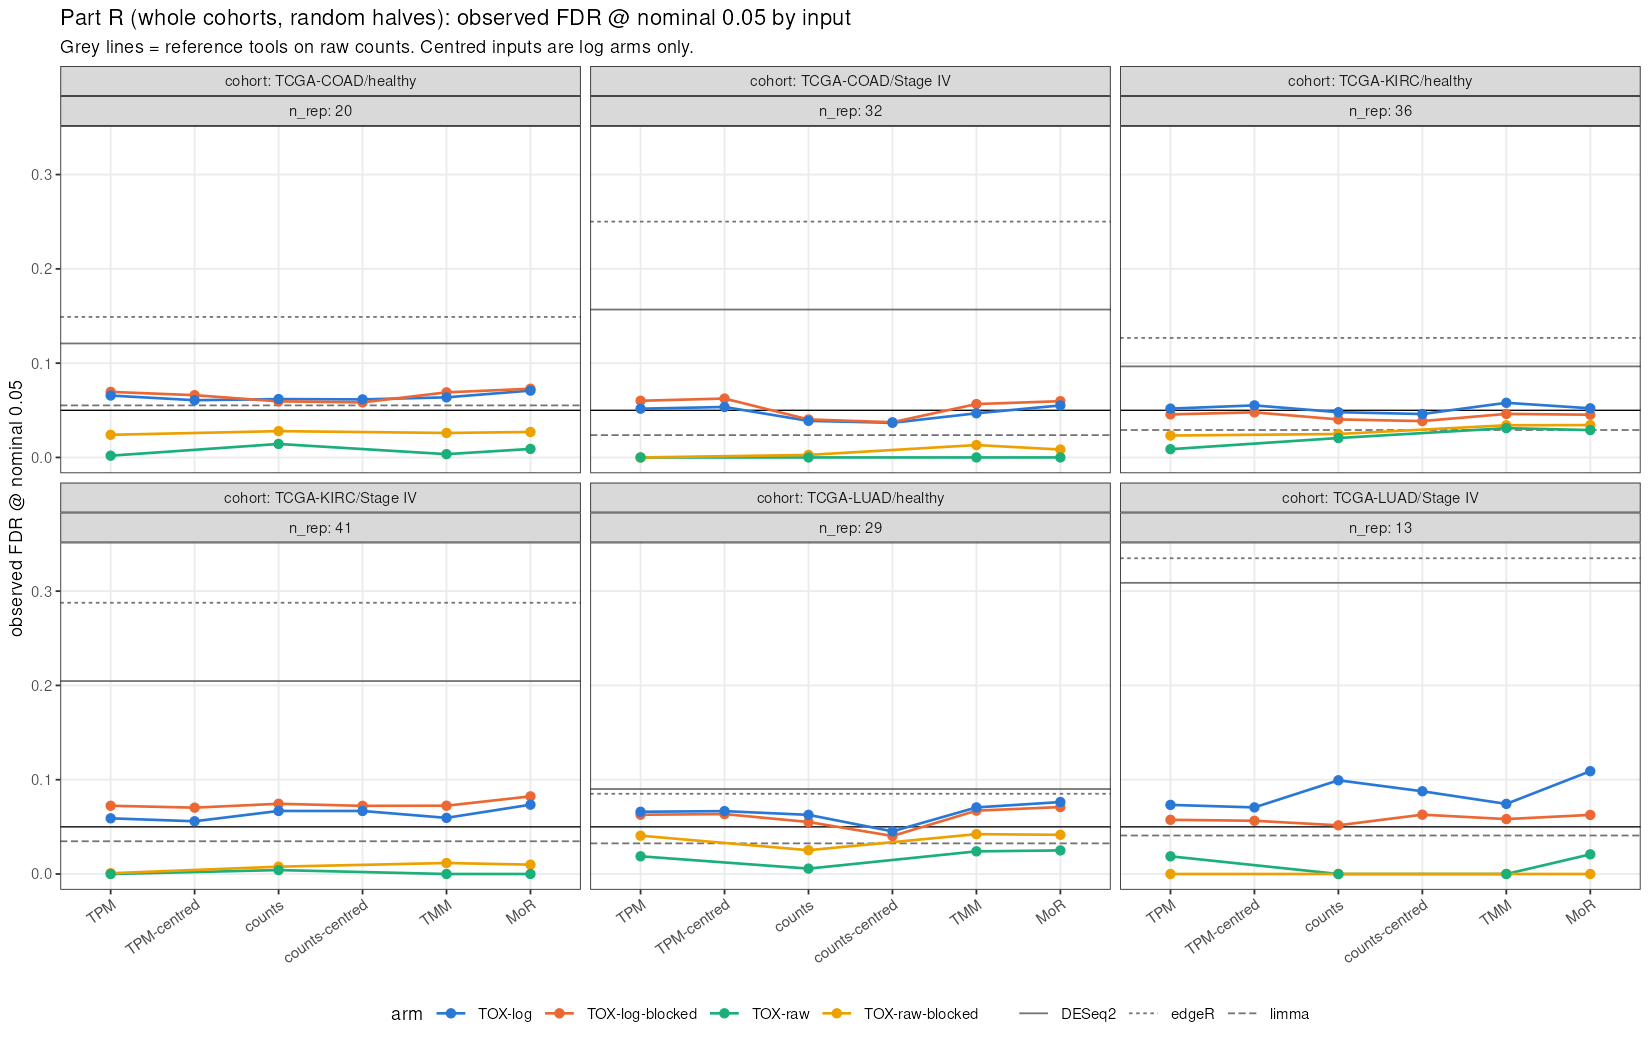
\includegraphics[width=\linewidth]{figures/grid_R_fdr_nom_05.png}
    \colbreak
    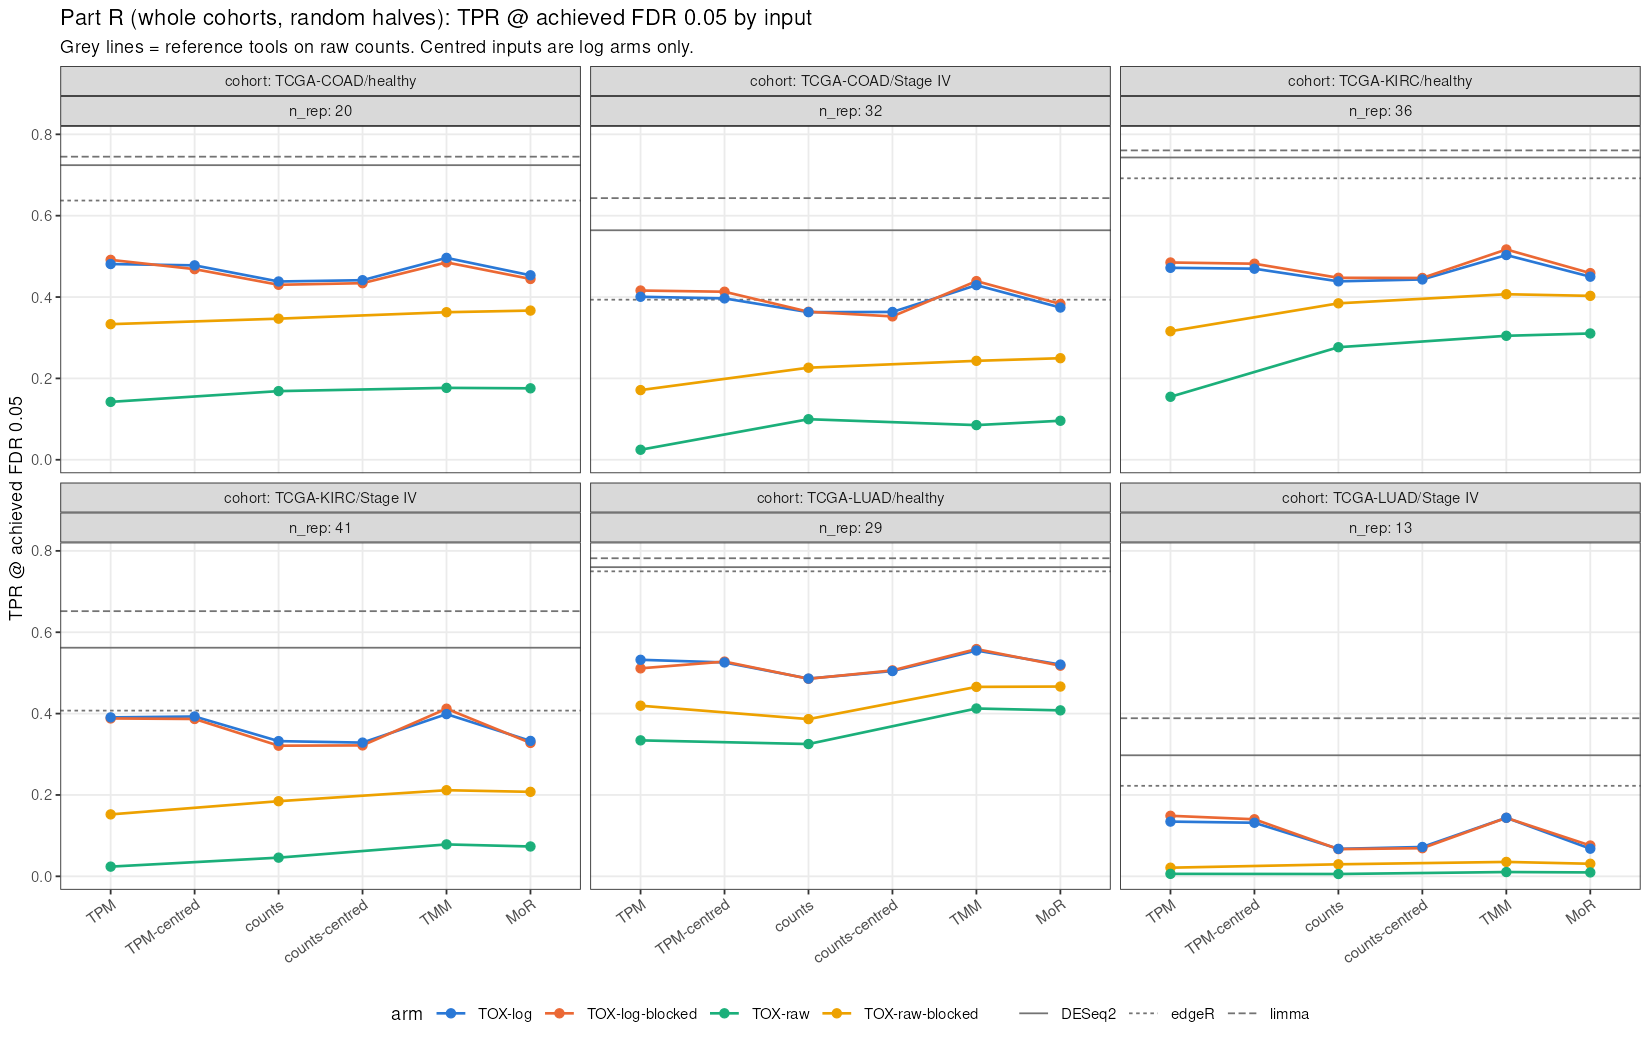
\includegraphics[width=\linewidth]{figures/grid_R_tpr_ach05.png}
  \end{twocols}
  {\centering\scriptsize\todo{presenter: confirm before showing; run of 19 Oct 2026}\par}
  \note{Added slide, not in the guide: the scalar (1-D) model's current results, so you see the starting
    point. Drop it in the 30-minute version.
    Left: observed FDR at nominal 0.05. Grey lines are the reference tools on raw counts; coloured lines
    are TOX arms on different input scales. Black horizontal line: nominal 0.05.
    Right: TPR at achieved FDR 0.05, i.e. power once each method is held to the same real FDR.
    Read it honestly: in these runs TOX-log keeps observed FDR closer to nominal than edgeR and DESeq2,
    but its power at matched FDR is below the reference tools in every cohort shown. TOX-raw is
    weaker still.
    Cohorts: TCGA-COAD, -KIRC, -LUAD, healthy and Stage IV. These are whole-cohort halves, 13 to 41
    samples per group. Real data at n = 3 and 5, the common case, has not been measured yet (planned
    as Part RS of the power test).
    Source: experiments/Noise\_Model\_Test/TCGA\_test/results/power\_out/ (run of 19 Oct 2026; plots
    re-rendered 21 Oct, same numbers). Full ranking view: backup B9.
    No multi-dimensional results exist yet; producing them is the project.}
\end{frame}

% ============================================================== data
% ---------------------------------------------------------------- 15
\section{Data}
\begin{frame}{Material and data}
  \begin{itemize}
    \item \textbf{available:} TCGA RNA-seq; healthy samples, one cohort per axis\\
          {\small (e.g.\ TCGA-KIRC, TCGA-LUAD, TCGA-STAD)}
    \item \textbf{available:} existing scripts for calibration and power
    \item \textbf{highly recommended:} a self-assembled multi-tissue dataset
    \item \textbf{not as main data:} mammal tissue set in \texttt{material/}
  \end{itemize}
  \note{TCGA is the guaranteed core and available now. In the TCGA design each cohort is one axis and
    only the healthy (normal-tissue) samples are used.
    Normal samples in TCGA are often taken adjacent to tumours and may not be perfectly healthy, and
    cohorts differ in how many normals they have. In the existing null-calibration run the healthy
    groups held 72 (kidney, TCGA-KIRC), 59 (lung, TCGA-LUAD) and 36 (stomach, TCGA-STAD) samples
    (null\_calibration\_summary.csv).
    Assembling a new multi-tissue dataset is highly recommended: not a strict requirement, but expected.
    Mammal dataset (material/kallisto\_sex\_data\_<Tissue>.tsv): 6 samples per tissue (8 in testis),
    so few per group once split. It contains real signal (sex differences), so a split is not a fully
    known null. Fine for exploration.}
\end{frame}

% ---------------------------------------------------------------- 16
\begin{frame}{Criteria for a new dataset}
  \begin{itemize}
    \item enough replicates per tissue to split (roughly $\ge 6$)
    \item independent samples across tissues
    \item homogeneous samples within a tissue
    \item count data available
    \item combined studies: same platform and quantification
  \end{itemize}
  \note{Independence has to be read from the methods sections: check whether tissues come from the same
    individuals. Different studies per tissue can be acceptable, because each axis is only compared
    within itself, provided the protocols are the same (sequencing platform and quantifier). Do not mix
    studies using different platforms or quantifiers. Some plant atlases use standardized extraction and
    processing protocols for exactly this reason. Within-tissue homogeneity must still be checked.
    TODO presenter: optional candidate list after checking. Do not name a dataset unless verified.}
\end{frame}

% ============================================================== students' work
% ---------------------------------------------------------------- 17
\section{First steps}
\begin{frame}{What you do, in tracks}
  \begin{itemize}
    \item \textbf{Track A:} dataset survey and assembly
    \item \textbf{Track B:} TOX on TCGA, calibration scripts
    \item \textbf{Track C:} reference tools, metrics, multi-tissue comparison
    \item \textbf{shared:} onboarding, final report
  \end{itemize}
  \note{Tracks are a suggestion; the number of students is not yet known, so we split on the go.
    Track C researches ideas for a multi-tissue comparison (omnibus tests, fry(), diffSpliceDGE(),
    others) to be discussed in the meetings. Choosing and justifying the comparison is your task;
    limitations are part of it.
    You work in R, with a provided Claude Code licence; check all generated code yourself.
    No Fortran knowledge needed: TOX is called through its R interface.}
\end{frame}

% ---------------------------------------------------------------- 18
\begin{frame}[fragile]{Repository tour}
  \begin{columns}[T,onlytextwidth]\begin{column}{0.47\textwidth}
    {\footnotesize
    \begin{tabular}{@{}l@{\hspace{0.8em}}l@{}}
      overview      & \texttt{README.md}, \texttt{concise\_project\_info.md} \\
      manuscript    & \texttt{misc/Tensor\_Omics\_Methods.pdf} \\
      R interface   & \texttt{rcpp/tensoromics\_functions.R} \\
      tests         & \texttt{test/mod\_test\_noise\_model*.f90} \\
      docs          & \texttt{experiments/Noise\_Model\_Test/docs/} \\
      test scripts  & \texttt{experiments/Noise\_Model\_Test/} \\
    \end{tabular}}
  \end{column}\hfill\begin{column}{0.5\textwidth}
\begin{code}[language=R, basicstyle=\ttfamily\scriptsize, numbers=none]
res <- tox_compute_noise_pvalues_pipeline_md(
  case_replicates    = list(leaf = case_leaf,
                            root = case_root),
  control_replicates = list(leaf = ctrl_leaf,
                            root = ctrl_root),
  max_pool_size      = 50000L)
\end{code}
  \end{column}\end{columns}
  \note{Repository: github.com/asishallab-group/Tensor-Omics, branch 145-empirical-noise-model (not merged
    into main). Test scripts: the submodule experiments/Noise\_Model\_Test (repository
    empirical-noise-model-testing): TCGA\_test/scripts/null\_calibration.R, power\_test.R,
    power\_report.R; Simulated\_data/scripts/calibration\_test.R and calibration\_test\_md.R (the
    multi-dimensional simulation; so far only a smoke run, no results).
    Docs: noise\_model\_current\_state.md describes the current model. Web documentation in doc/.
    Build: ./build.sh, then source("rcpp/tensoromics\_functions.R"). Unit tests: ./test\_runner.sh.
    The call: one matrix per axis, samples x genes, row names = sample IDs, identical gene columns.
    max\_pool\_size has no default in the R function; 50000 is never reached.
    Show where to start reading and where to run something; no live coding.}
\end{frame}

% ---------------------------------------------------------------- 19
\begin{frame}{First two weeks}
  \relax  {\centering\resizebox{0.97\linewidth}{!}{% F7: first two weeks, shared tasks and parallel tracks (a suggestion; tracks decided on the go)
\begin{tikzpicture}[font=\scriptsize,
    task/.style={draw=none, fill=#1, rounded corners=2pt, align=left, inner sep=3.5pt,
                 text=thbink, anchor=west, minimum height=0.62cm},
    trk/.style={anchor=east, font=\scriptsize\bfseries, text=thbink, align=right}]
  % week grid
  \foreach \w/\x in {1/0,2/6.2} {
    \node[anchor=south, font=\footnotesize\bfseries, text=thbprimary] at (\x+3.1,0.35) {week \w};
  }
  \draw[thbline] (6.1,0.4) -- (6.1,-3.65);
  \node[trk] at (-0.1,-0.1) {everyone};
  \node[trk] at (-0.1,-1.15) {Track A\\[-2pt]{\tiny datasets}};
  \node[trk] at (-0.1,-2.2) {Track B\\[-2pt]{\tiny TOX on TCGA}};
  \node[trk] at (-0.1,-3.25) {Track C\\[-2pt]{\tiny reference tools}};
  \node[task=thbtint, text width=5.6cm] at (0,-0.1) {(1) set up R, build TOX, run the example call};
  \node[task=thbtint, text width=5.6cm] at (6.2,-0.1) {(2) read: normalization, edgeR / limma / DESeq2};
  \node[task=accentcol!25, text width=11.8cm] at (0,-1.15) {(4) survey candidate multi-tissue datasets $\rightarrow$ one-page comparison against the criteria};
  \node[task=ctrlcol!18, text width=5.6cm] at (0,-2.2) {(3) explore TCGA: library sizes, filtering, mean--variance};
  \node[task=ctrlcol!18, text width=5.6cm] at (6.2,-2.2) {(5) reproduce one scalar calibration plot};
  \node[task=casecol!22, text width=11.8cm] at (0,-3.25) {read on multi-tissue comparisons (omnibus tests, \texttt{fry()}, \texttt{diffSpliceDGE()}, \ldots): what does each test?};
  \node[anchor=north east, text=thbmuted] at (12.0,-3.75) {end of week 2: everyone runs the pipeline; dataset decision date agreed};
\end{tikzpicture}
}\par}
  \note{(1) set up R, build or install TOX, run the example call; (2) read: RNA-seq normalization and
    the three tools; (3) explore TCGA: library sizes, filtering, mean-variance plot; (4) Track A: a
    one-page comparison of candidate datasets against the criteria; (5) reproduce one existing
    calibration plot of the scalar model.
    The aim: everyone can run the pipeline, and we agree on the dataset decision date.}
\end{frame}

% ---------------------------------------------------------------- 20
\section{Outlook}
\begin{frame}{Outlook}
  \relax  {\centering
  \begin{tikzpicture}[font=\footnotesize]
    \node[ph=thbtint, minimum width=3.0cm] (a) at (0,0) {onboarding\\and data};
    \node[ph=nullcol!30, minimum width=2.6cm, right=0.15cm of a] (b) {calibration};
    \node[ph=obscol!25, minimum width=2.6cm, right=0.15cm of b] (c) {power};
    \node[ph=casecol!25, minimum width=2.6cm, right=0.15cm of c] (d) {parameter\\exploration};
    \node[ph=accentcol!25, minimum width=2.2cm, right=0.15cm of d] (e) {final\\report};
    \node[anchor=north, text=thbmuted] at (a.south) {months 1--2};
  \end{tikzpicture}\par}
  \vspace{1.2em}
  \begin{itemize}
    \item calibration first, power as time allows
    \item about 180\,h per student (6 ECTS): a guideline, not a target
  \end{itemize}
  \note{Do as much as possible. Calibration comes first; power as time allows.
    180 hours is the university guideline for 6 ECTS, not a hard target.}
\end{frame}

% ============================================================== close
% ---------------------------------------------------------------- 21
\begin{closing}[Questions?]
  \item the noise model decides every DE result
  \item TOX: empirical null; check where its assumptions fail
  \item your work: calibration and power, in parallel tracks
\end{closing}

% ============================================================== backup
\thbbackup

% ---------------------------------------------------------------- B1
\begin{frame}{B1: Null construction, worked example for $d = 2$}
  \begin{itemize}
    \item pool per axis and side: $k$ genes $\times$ $n$ replicates residuals
    \item e.g.\ $k = 20$, $n = 3$: 60 per side, $S_a = 60 \times 60 = 3600$ pairs
    \item joint space $S_1 S_2 \approx 1.3 \times 10^7$ $\Rightarrow$ sampled
    \item weights $w_a = 1/\mathrm{Var}_{\mathrm{null}}(a)$
    \item check: $\mathrm{E}[D^2_{\mathrm{std},0}] = $ number of axes with $w_a > 0$
  \end{itemize}
  \note{k counts genes; each gene contributes n residuals. 20 genes at 3 replicates give 60 residuals
    per side (more if the pool grows adaptively). Atoms per axis: every case residual paired with every
    control residual. The joint space is the product over axes, far above the enumeration cap
    (enum\_max\_product, currently 1e5), so d = 2 is sampled.
    Sanity check: each gene's residuals sum to zero, so the pools have mean zero and
    E[w\_a v\_a^2] = w\_a Var\_null(a) = 1 for every axis with positive weight. A degenerate axis
    (zero pool variance) gets weight 0.
    Example numbers use the current defaults, which may change.}
\end{frame}

% ---------------------------------------------------------------- B2
\begin{frame}{B2: Three p-value paths and resolution}
  \begin{itemize}
    \item enumeration: all combinations, while $\prod_a S_a \le$ cap
    \item systematic stride sampling (default): deterministic, no seed
    \item random sampling: classical Monte Carlo
    \item floor $1/(M+1)$; current default $M = 20{,}000$
    \item $M$ set by the gene count under BH, not by $d$
  \end{itemize}
  \note{method\_used per gene: 0 enumerated, 1 systematic, 2 RNG. Enumeration also uses (count+1)/(m+1),
    so its floor is 1/(number of atoms + 1), tiny but not zero.
    Systematic: each pool is walked with a fixed stride coprime to its size; (1+B)/(M+1) is then an
    approximation of the exact tail rather than a Monte-Carlo p-value; compare both arms on the mock null.
    Resolution: a gene at the floor is rejected only if its BH rank reaches p\_floor * G / q. At
    G = 20000 and q = 0.05 that is about 20 genes tied at the floor before any is rejected. The tail
    probability is one-dimensional, so its standard error sqrt(p(1-p)/M) does not depend on d.
    Optional Besag-Clifford stopping (n\_exceed\_target) exists but is off by default.}
\end{frame}

% ---------------------------------------------------------------- B3
\begin{frame}{B3: Parameters (current defaults, may change)}
  \relax  {\small
  \begin{tabular}{lll}
    \toprule
    \thbhead{Argument} & \thbhead{Current default} & \thbhead{Meaning} \\
    \midrule
    \texttt{k\_start}, \texttt{k\_step}, \texttt{k\_max} & 20, 1, 50 & neighbour genes \\
    \texttt{tau} & 0.1 & stop growing the pool \\
    \texttt{norm\_method} & 1 (log2) & 0 = linear \\
    \texttt{beta\_centre} & 0 & 1 = subtract per-axis median $\hat\beta$ \\
    \texttt{n\_draws\_max}, \texttt{sampling\_mode} & 20000, 0 & $M$; systematic \\
    \bottomrule
  \end{tabular}}
  \note{All values from the R wrapper tox\_compute\_noise\_pvalues\_pipeline\_md and subject to change.
    Further arguments: enum\_max\_product = 1e5, n\_exceed\_target = 0 (off), seed = 42 (RNG path only),
    null\_method must be 0, check\_axis\_samples = TRUE, max\_pool\_size has no default.
    beta\_centre must be 0 if the data were already normalized on the R side, or the data are centred twice.
    Say "k is a parameter" until the defaults are decided.}
\end{frame}

% ---------------------------------------------------------------- B4
\begin{frame}{B4: Why scale residuals by $1/\sqrt{n}$}
  \begin{itemize}
    \item observed: a difference of \textbf{means} over $n$ replicates
    \item one residual: single-observation scale
    \item $\mathrm{Var}(\bar x) = \sigma^2 / n$ $\Rightarrow$ scale by $1/\sqrt{n}$
    \item without it: null too wide, test conservative
    \item caveat: fixes the variance, not the \emph{shape}
  \end{itemize}
  \note{The mean of n residuals has variance sigma\^{}2/n; scaling one residual by 1/sqrt(n) matches that
    variance. But the distribution of a mean is more Gaussian than that of a single residual; scaling
    does not change the shape. The bootstrap module resamples means and so gets the shape too.}
\end{frame}

% ---------------------------------------------------------------- B5
\begin{frame}{B5: Why not a joint neighbourhood in $d$ dimensions?}
  \begin{itemize}
    \item joint kNN: neighbours must match on \emph{all} axes at once
    \item distances grow with $d$: fewer good matches
    \item tissue-specific genes match poorly on at least one axis
    \item needed only if axes share samples (out of scope)
  \end{itemize}
  \note{Per-axis 1-D matching gives each axis neighbours at the right level. A joint neighbourhood would
    be required if samples were paired across axes (the null would need whole d-vectors from one sample);
    that case is out of scope and guarded by the sample-ID check.}
\end{frame}

% ---------------------------------------------------------------- B6
\begin{frame}{B6: Glossary}
  \relax  {\small
  \begin{tabular}{@{}ll@{}}
    axis & one tissue (or cohort) dimension of a gene's effect vector \\
    $\hat\beta_a$ & case minus control mean on axis $a$ \\
    $D$, $D_{\mathrm{std}}$ & effect size; standardized test statistic \\
    residual & replicate minus its group mean \\
    neighbourhood & genes with similar group mean, per axis and side \\
    calibration & FPR at a threshold equals the threshold \\
    FDR, TPR & false discoveries among calls; share of true effects found \\
  \end{tabular}}
\end{frame}

% ---------------------------------------------------------------- B7 (existing results)
\begin{frame}{B7: Scalar model, mock-null calibration on TCGA}
  \relax  {\centering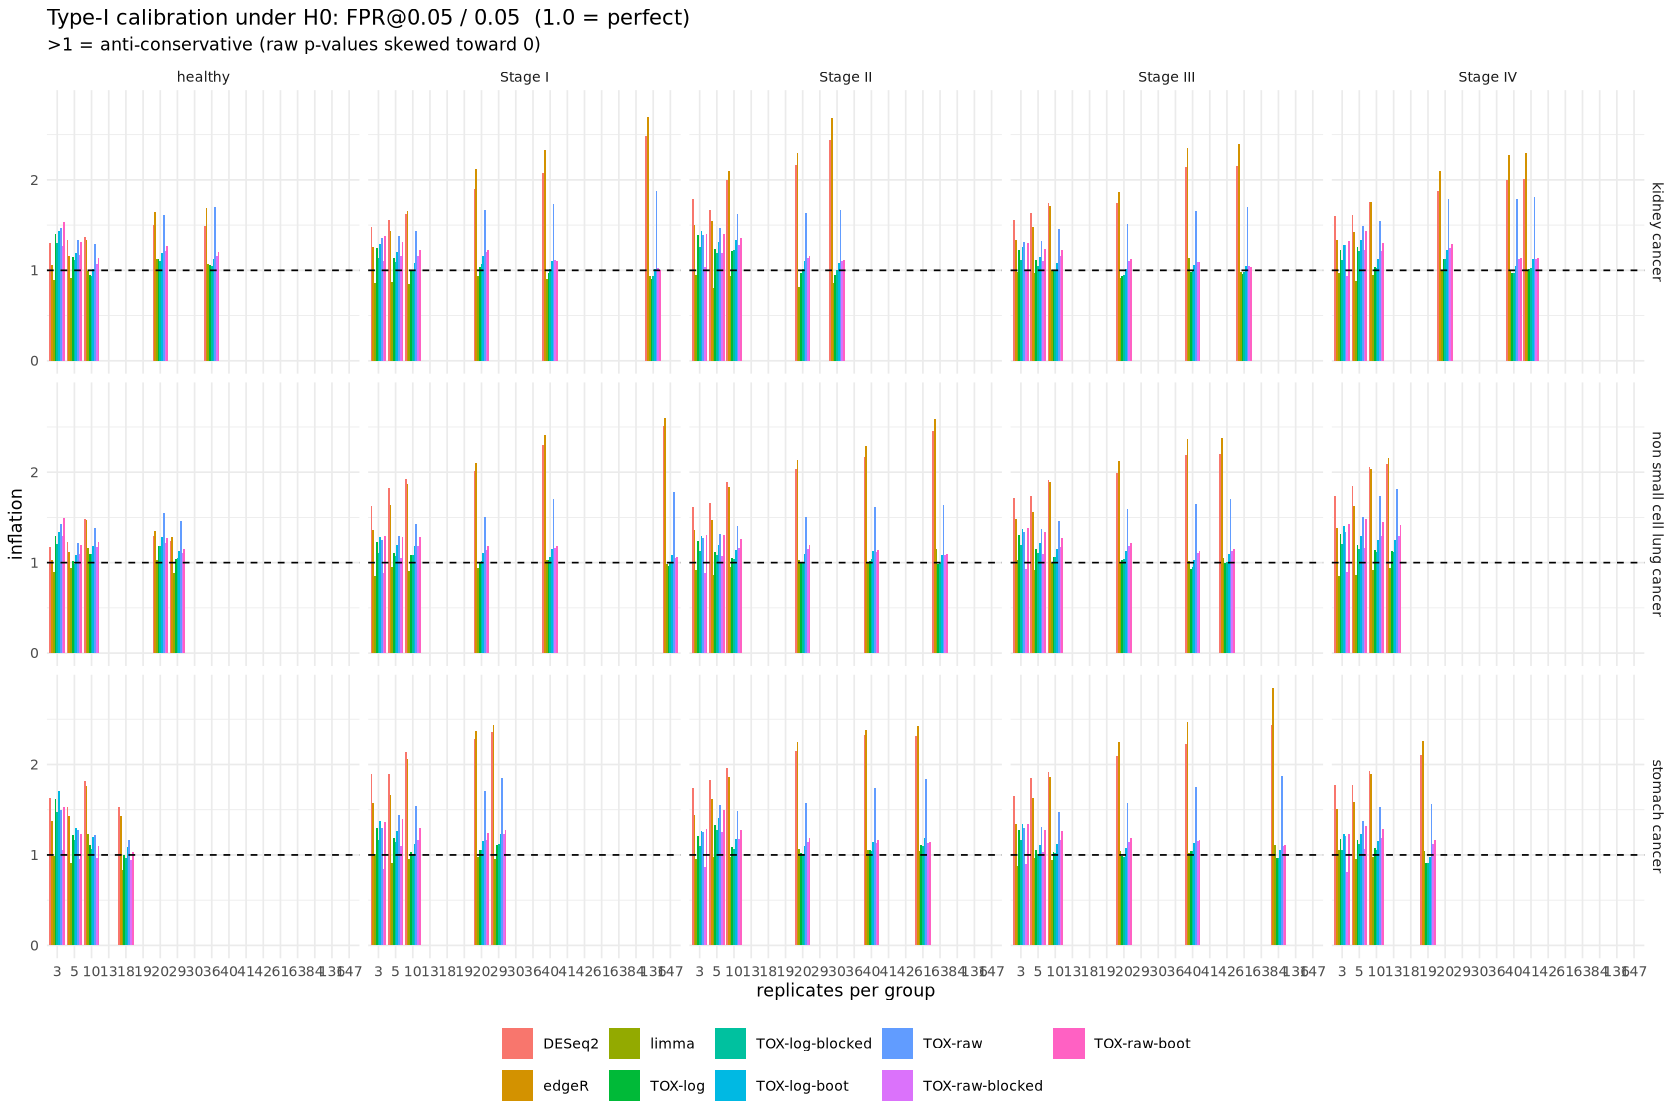
\includegraphics[height=0.78\textheight]{figures/null_fpr_inflation.png}\par}
  \note{FPR at 0.05 divided by 0.05 on random halves of one group (1.0 = perfect), per cohort, stage,
    replicates per group. Scalar model arms and the reference tools.
    Source: TCGA\_test/results/null\_calibration/plots/null\_fpr\_inflation.png (run of 30 Sep 2026).
    TODO presenter: confirm before showing.}
\end{frame}

% ---------------------------------------------------------------- B8 (existing results)
\begin{frame}{B8: Scalar model, simulated counts (Part P)}
  \relax  {\centering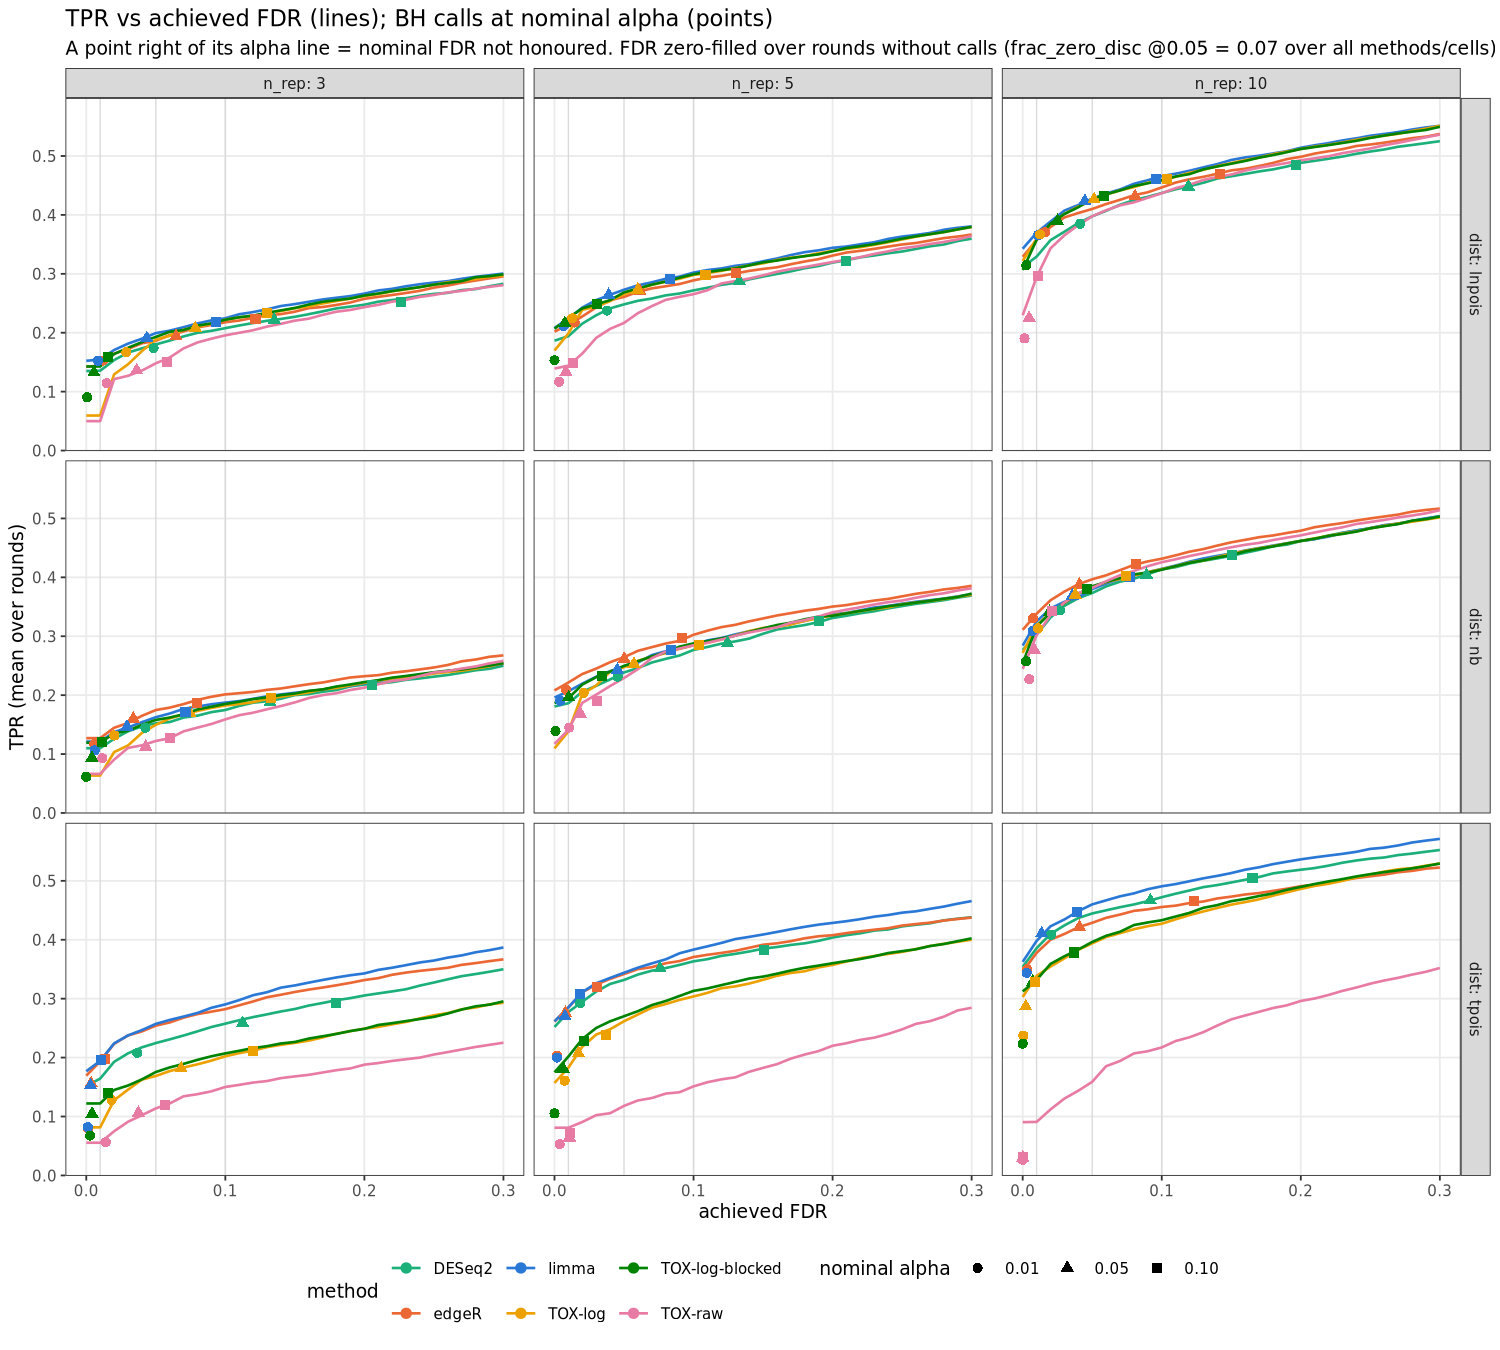
\includegraphics[height=0.78\textheight]{figures/fdr_tpr_curves.png}\par}
  \note{TPR against achieved FDR on simulated counts (negative binomial, log-normal Poisson, tpois),
    n = 3, 5, 10 replicates; points = BH calls at nominal alpha.
    Source: TCGA\_test/results/power\_out/fdr\_tpr\_curves.png (run of 19 Oct 2026).
    TODO presenter: confirm before showing.}
\end{frame}

% ---------------------------------------------------------------- B9 (existing results)
\begin{frame}{B9: Scalar model, Part R precision--recall}
  \relax  {\centering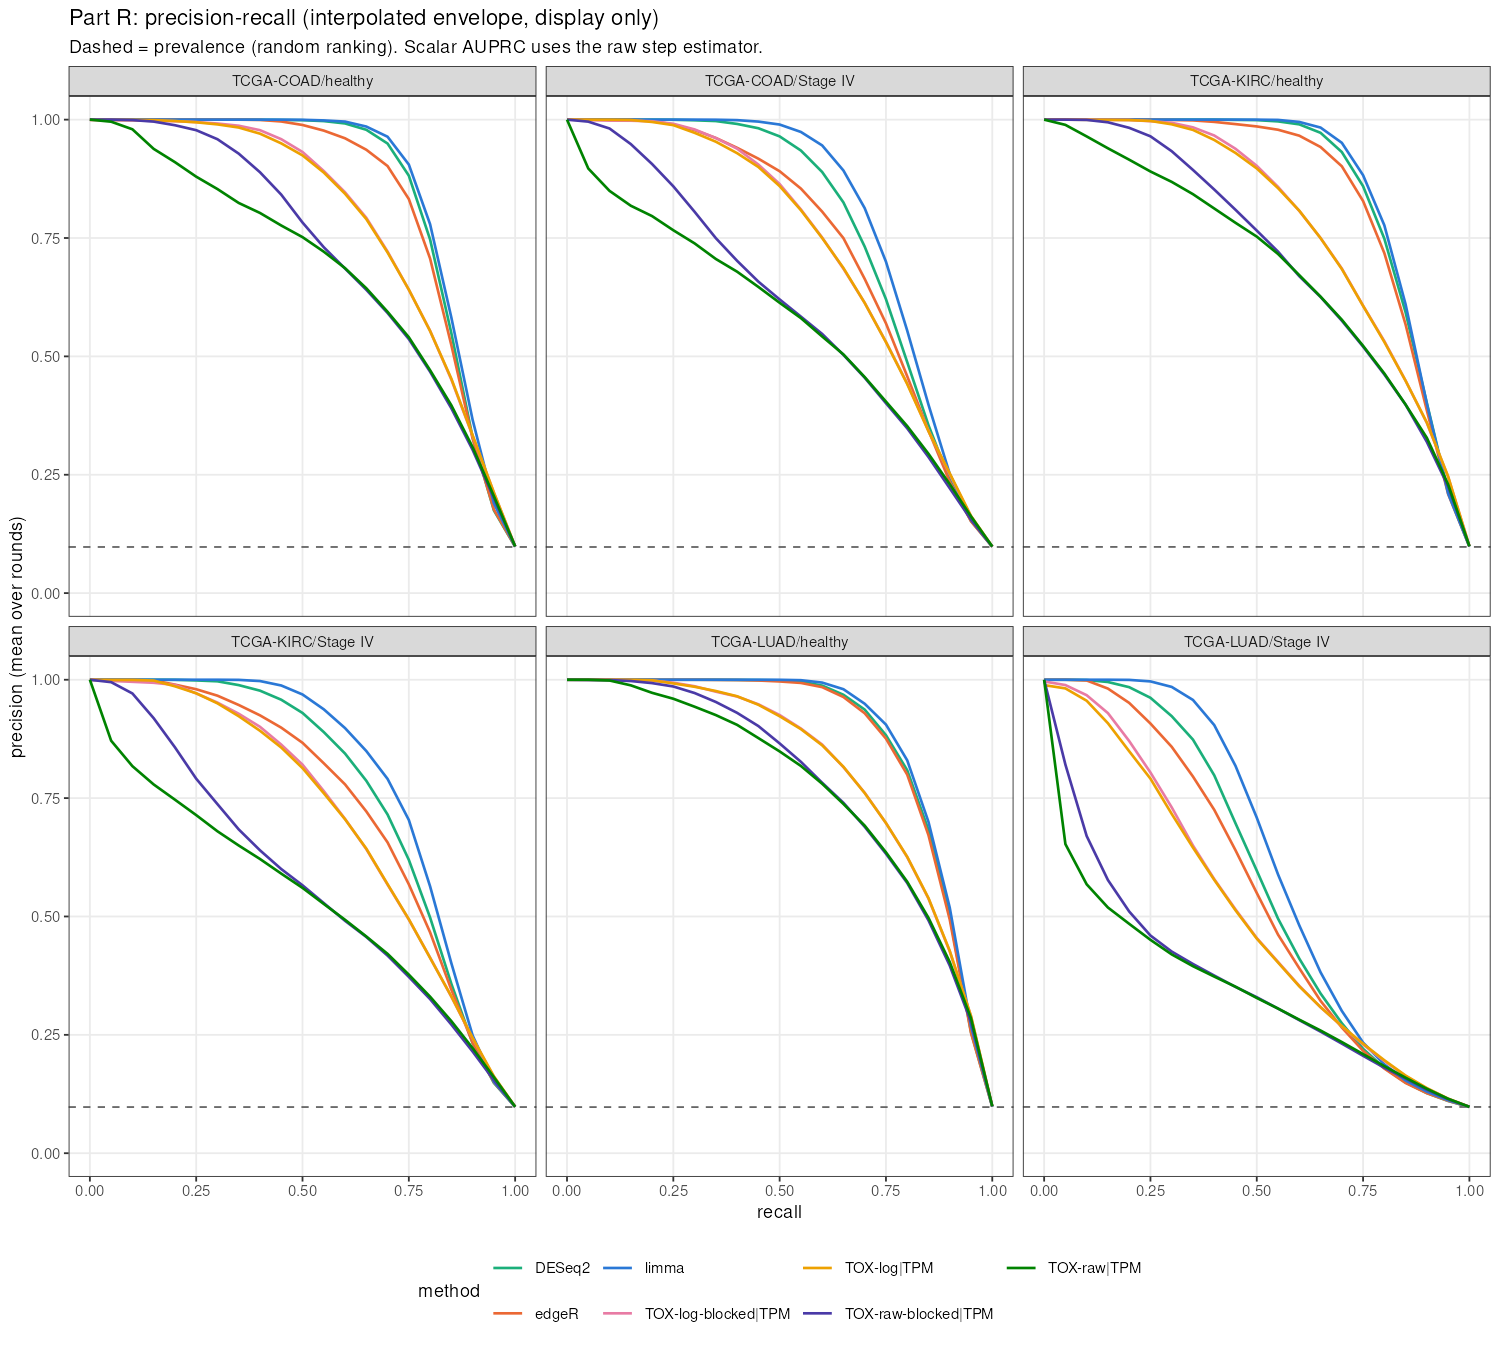
\includegraphics[height=0.78\textheight]{figures/pr_curves_R.png}\par}
  \note{Same Part R run as slide 14b, but over the whole ranking instead of one operating point:
    precision against recall, averaged over 20 rounds; dashed line = prevalence (random ranking).
    TOX-log stays below limma, edgeR and DESeq2 over most of the recall range; the raw arms are lower
    still, most clearly in the Stage IV cohorts.
    Source: TCGA\_test/results/power\_out/pr\_curves\_R.png. TODO presenter: confirm before showing.}
\end{frame}

\end{document}
